\subsection{Experimental setup}
\begin{wraptable}{h}{7cm}
\caption{Properties of iodine.}
\begin{tabular}{| l | r |}
    \hline
    atomic mass   & $126.9$ u \\
    \hline
    melting point & $113.7^{\circ}$C \\
    \hline
    boiling point & $184.3^{\circ}$C \\ 
    \hline
    density & $4.94 \text{gcm}^{-3} $ \\
    \hline
    valance elecrons & 7 \\
    \hline
    electronegativity & 2.66 \\
    \hline
    atomic radius & 140 pm \\
    \hline
\end{tabular}
\label{tab:iodine}
\end{wraptable}


Our experimental setup is as follows \cite{versuchsanleitung}:
First we will have a construction such that we can measure the 
the peaks of a given natrium-, mercury and halogenlamp, you 
can see the setup in figure~\ref{fig:const1}.
After having measured the spectra we will continue and append
the iodine-pipe into the setup, see figure~\ref{fig:const2}.
The pipe is 50 cm long and its diameter is 4 cm. Its inner 
vapour pressure is 0.5 Torr. It will be 
inserted between the lamp and the spectroscope, which is on 
the right side. Here we give some details \cite{weisstein} 
about the iodine molecule, see table~\ref{tab:iodine}.

\begin{wrapfigure}{r}{0.50\textwidth}
  \begin{center}
    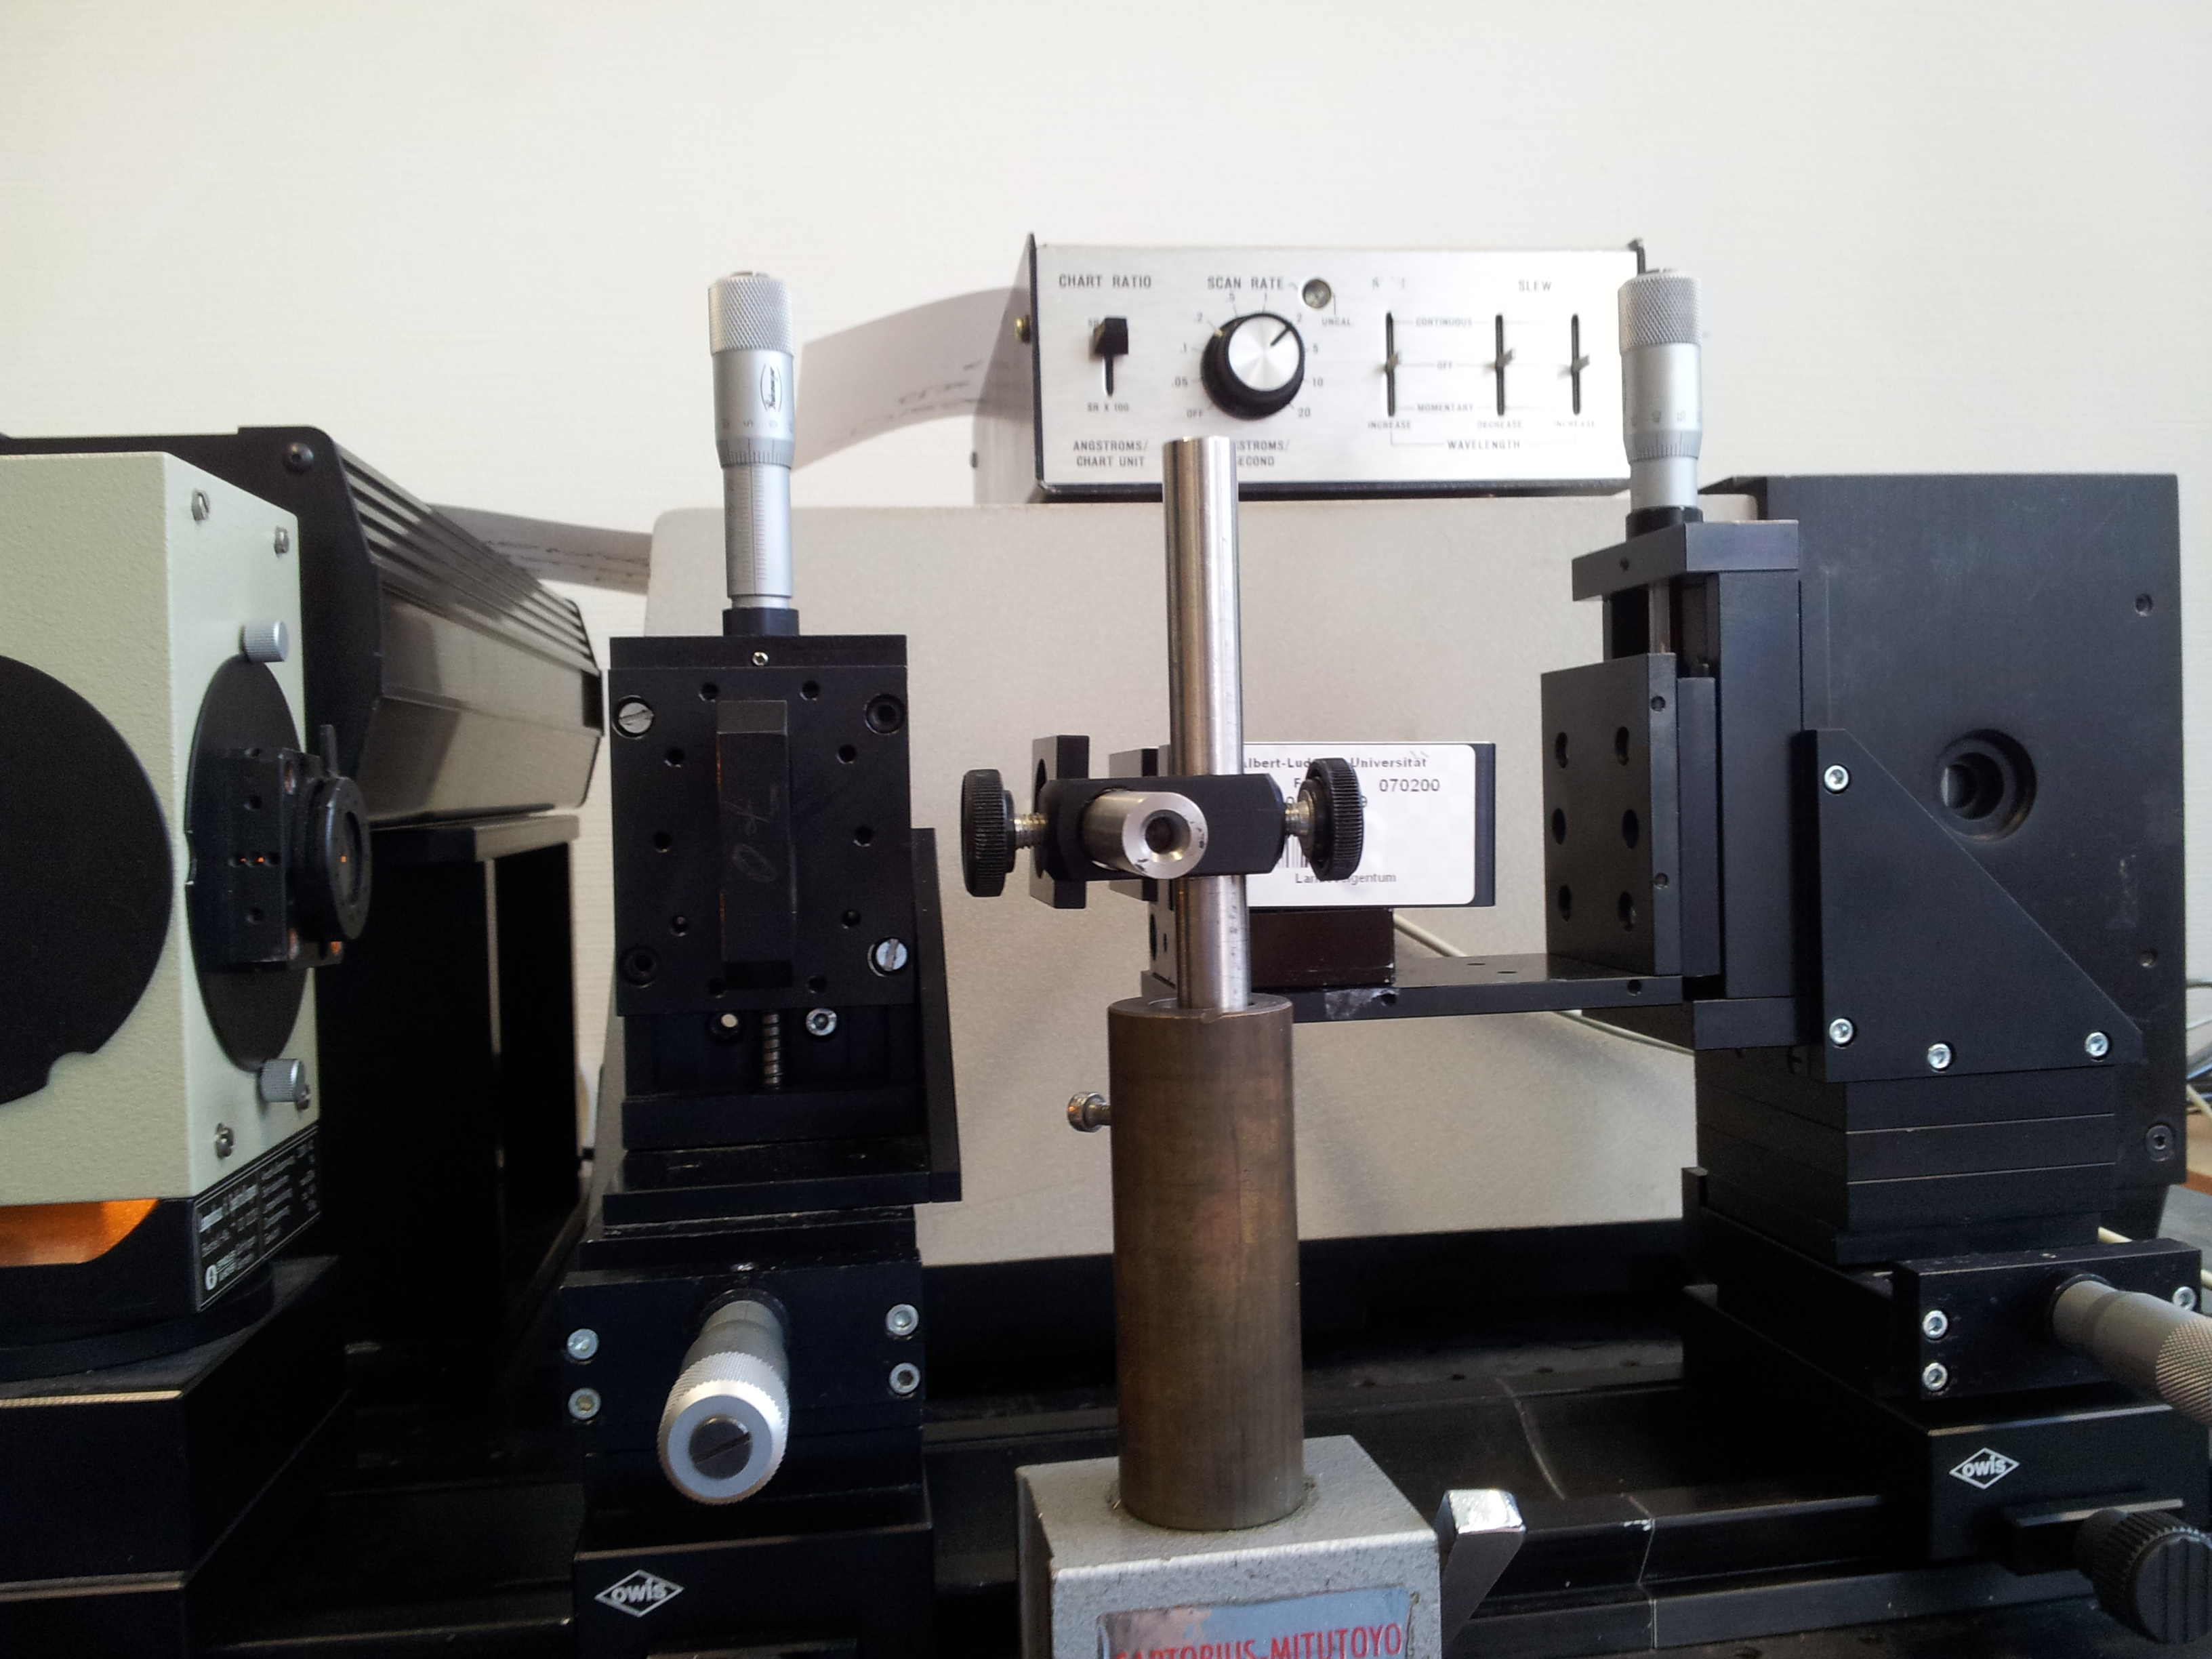
\includegraphics[width=0.48\textwidth]{pics/const1}
  \end{center}
\caption{Photography of the experimental setup when we measure
    the spectra of the given lightsources. The little white box is
    the spectroscope.} 
 \label{fig:const1}

\end{wrapfigure}
\subsubsection{CCD-Spectroscope}
The Device itself was invented 1969 at the 
\textit{AT\&T Bell Labs}. It is a Charge Couple Device (CCD) and it uses
the photoeffect for translating the information of the wavelength
of the photon into a potential difference, which can be saved
in terms of condensators. So effectively the number of electrons
resample the number of incoming photons.
It consists of a high-sensitivity 2048-element CCD array of sony 
(see table~\ref{tab:ccd} for more details) and 


It is very widely used
both in scientific and industrial usage.
We use the \textit{USB2000+} of the company \textit{ocean optics}
\cite{versuchsanleitung}. The spectroscope uses a lattice in order
to split the light beam in its wavelengths. 
The opening is 20 $\mu m$ and the wavelengths which will be
detected are 421 to 617 nm with a spectral resolution of 0.6 nm.
After detecting 
the photons they will be visualized at the computer, where we
can save the given spectrum to a file within the given software
\textit{SpectraSuite}.
\begin{wrapfigure}{r}{0.50\textwidth}
\caption{Setup with iodinepipe.} 
  \begin{center}
    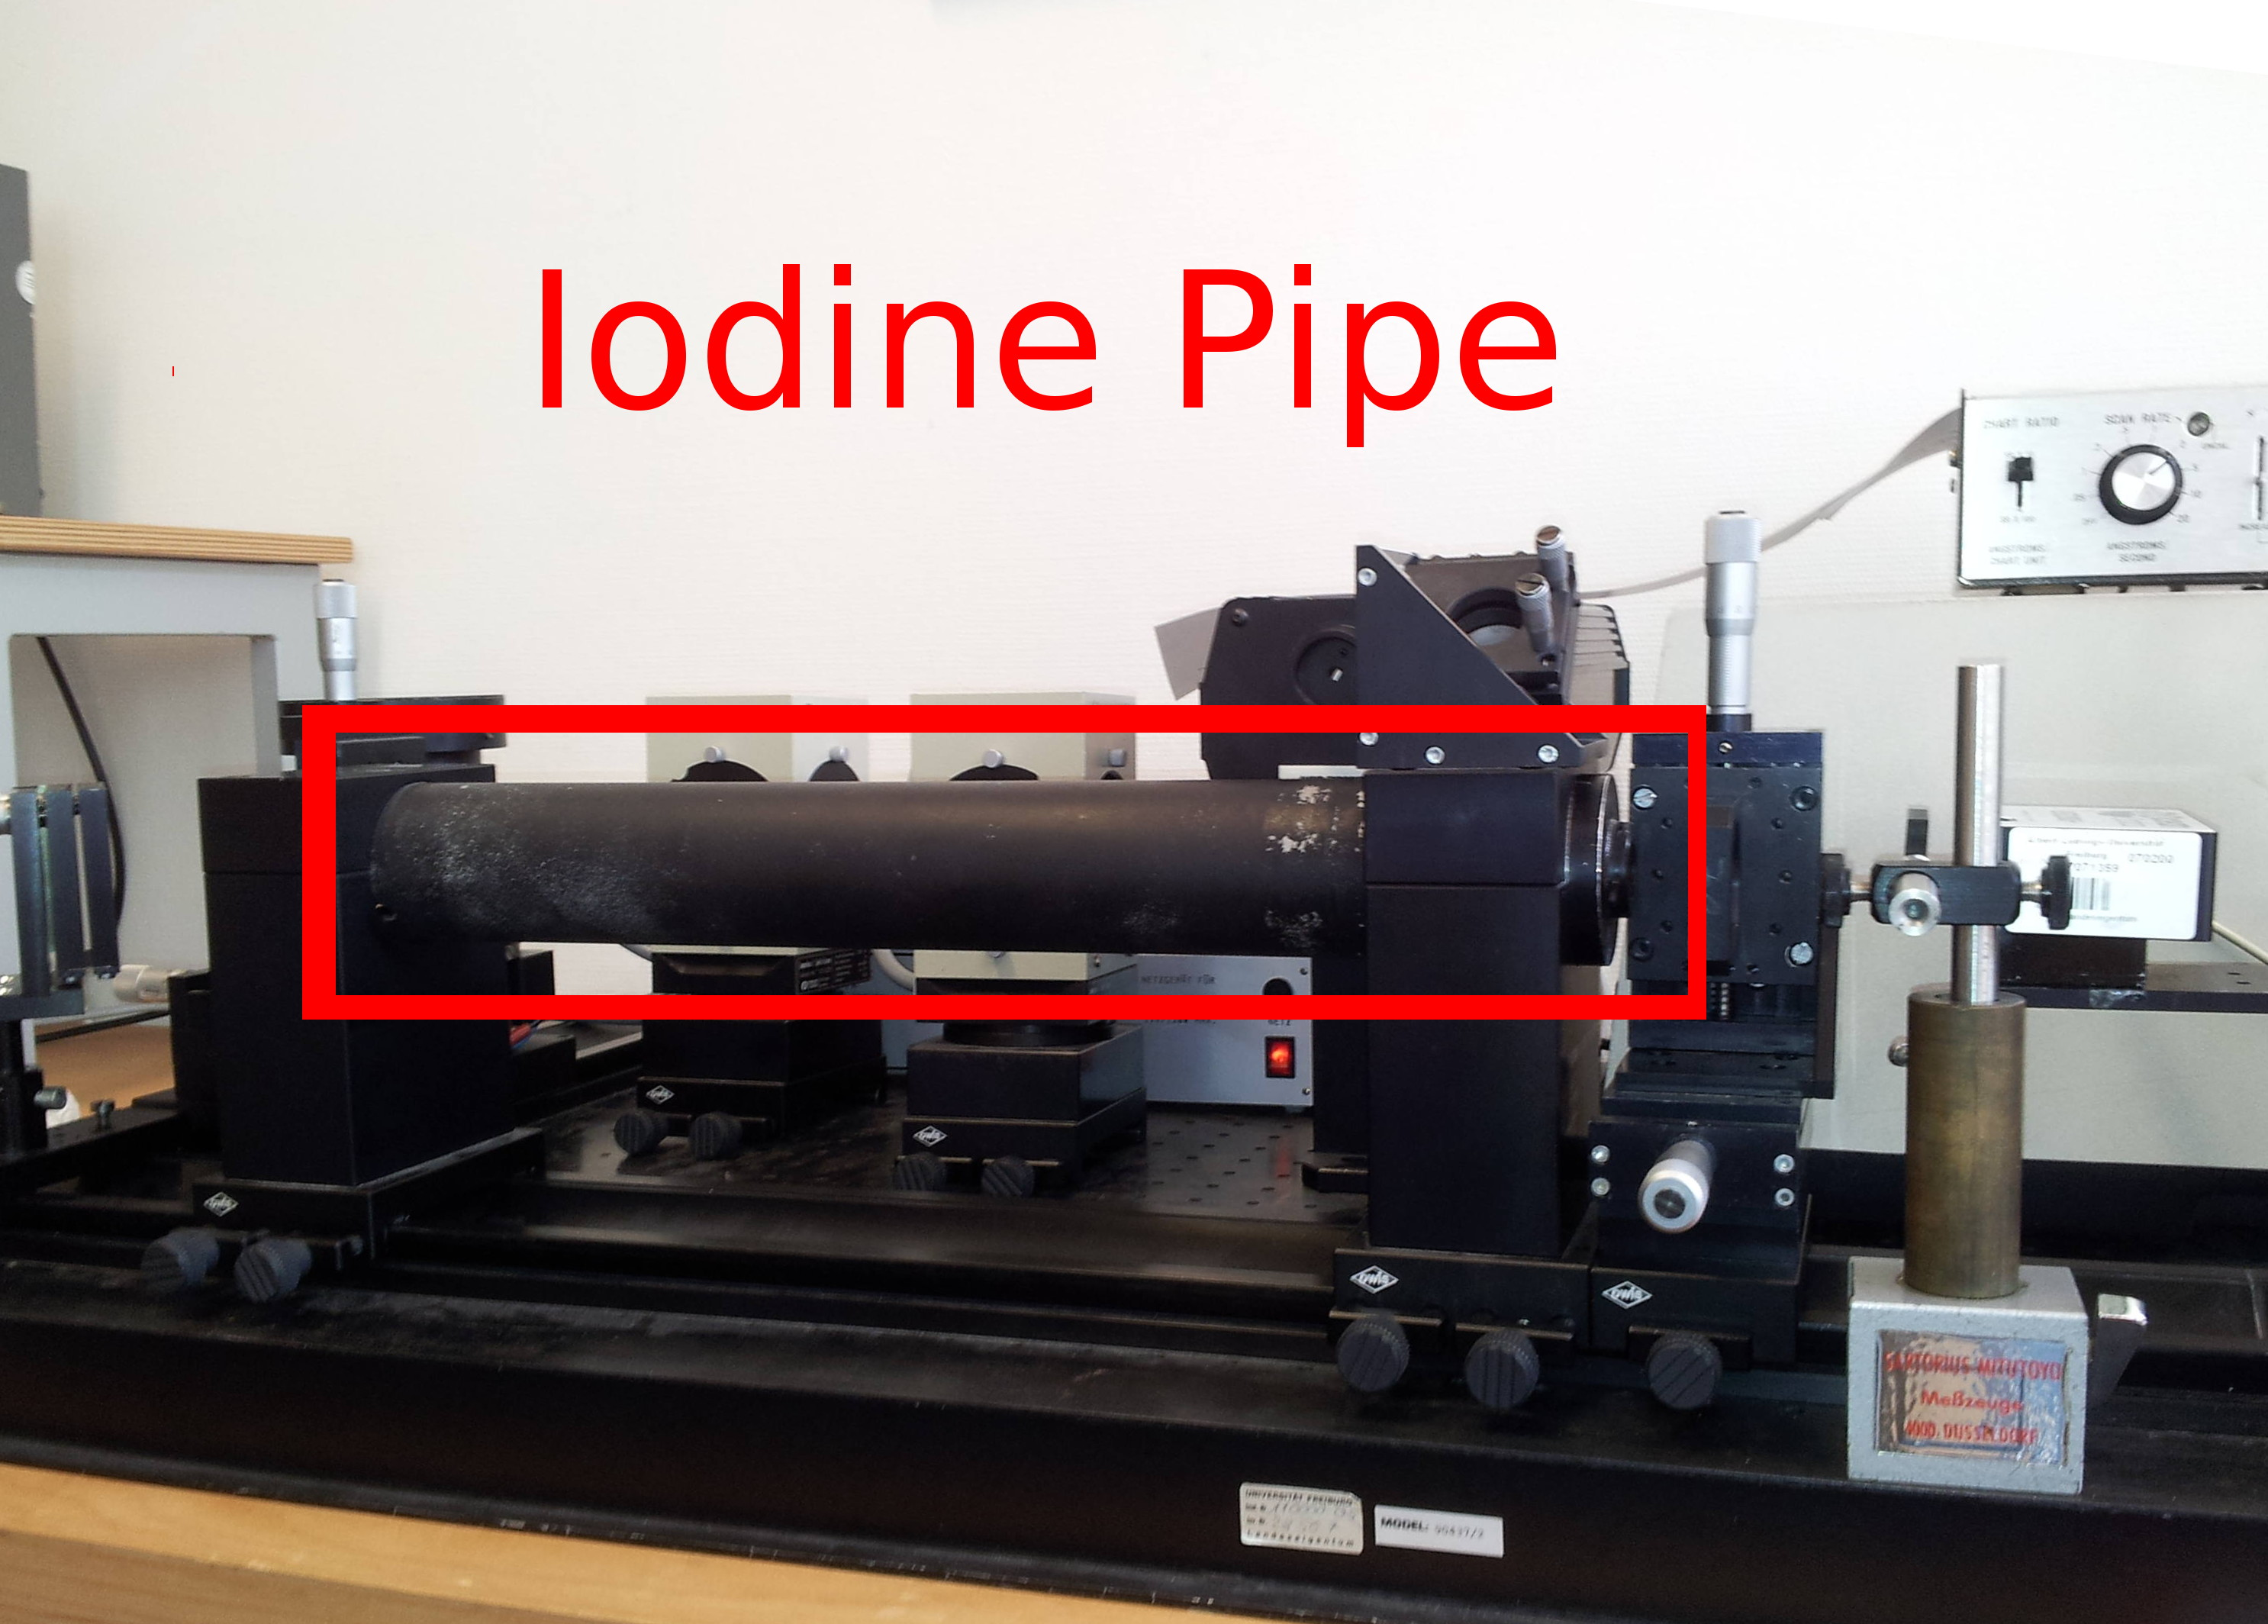
\includegraphics[width=0.48\textwidth]{pics/const2}
  \end{center}
 \label{fig:const2}
  \vspace{+10pt}
\end{wrapfigure}

\begin{wraptable}{h}{7cm}
    \caption{Specifications of the  CCD Camera \textit{usb2000+} \cite{usb2000_site}.}
\begin{tabular}{| l | l |}
    \hline
    Dimensions & 89.1 mm x 63.3 mm x 34.4 mm \\ 
    \hline
    Detector & Sony ILX511B (2048-element \\
             & linear silicon CCD array) \\  
    \hline
    Range & 200-1100 nm \\ 
    \hline
    Pixels: & 2048 pixels \\ 
    \hline
    Pixelsize & 14 µm x 200 µm \\ 
    \hline
    Optical resolution: & 0.3-10.0 nm \\ 
    \hline
\end{tabular}
\label{tab:ccd}
\end{wraptable}


sample textsample textsample textsample textsample textsample text
sample textsample textsample textsample textsample textsample text
sample textsample textsample textsample textsample textsample text
sample textsample textsample textsample textsample textsample text
ample textsample textsample textsample textsample textsample text
sample textsample YYYextsample textsample textsample textsample text
\subsubsection{Spectra of light sources}
In this experiment we will use the nearly continuos spectrum of
the halogenlamp, but before we will calibrate the spectroscope
with the spectra of the other lamps as following:
\par
\begin{wrapfigure}{r}{0.50\textwidth}
  \begin{center}
    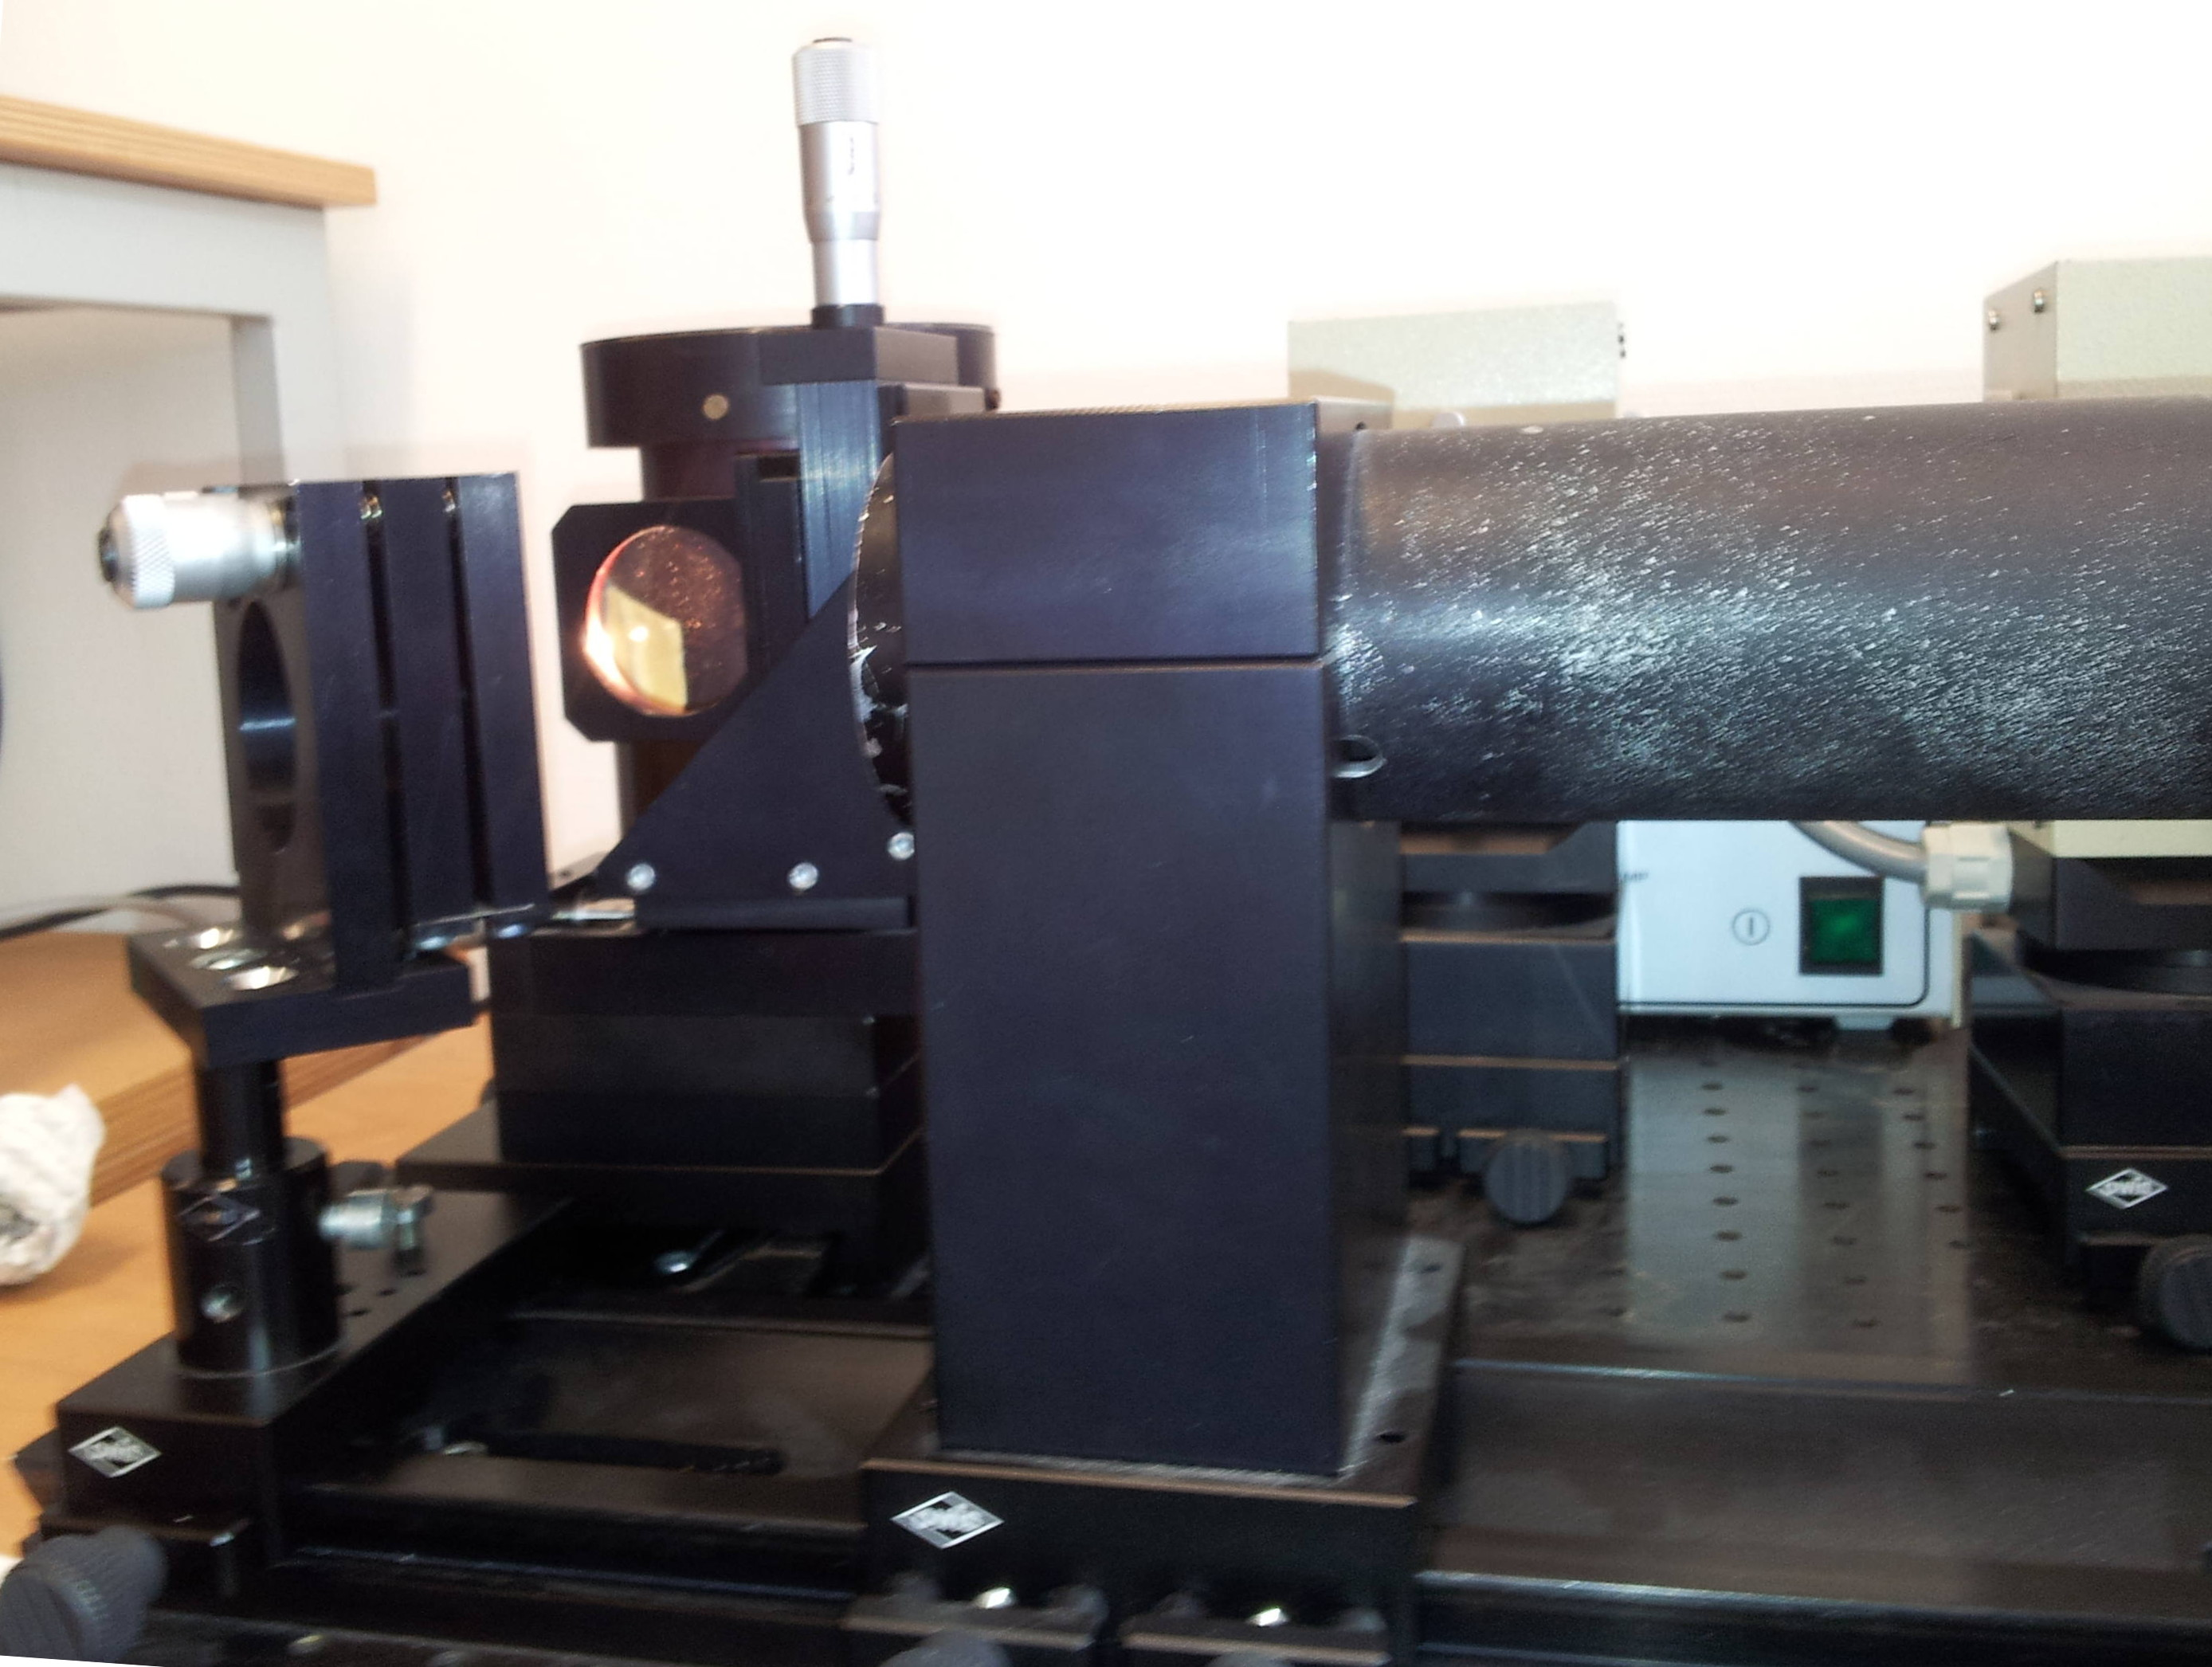
\includegraphics[width=0.47\textwidth]{pics/const4}
  \end{center}
\caption{Photography of the experiment.} 
  \vspace{-10pt}
 \label{fig:const4}

\end{wrapfigure}

sample textsample textsample textsample textsample textsample text
sample textsample textsample textsample textsample textsample text
sample textsample textsample textsample textsample textsample text
sample textsample textsample textsample textsample textsample text
sample textsample textsample textsample textsample textsample text
sample textsample textsample textsample textsample textsample text
\begin{SCfigure} 
\caption{On this photography you can recognize very 
    clearly the spectroscope!!} 
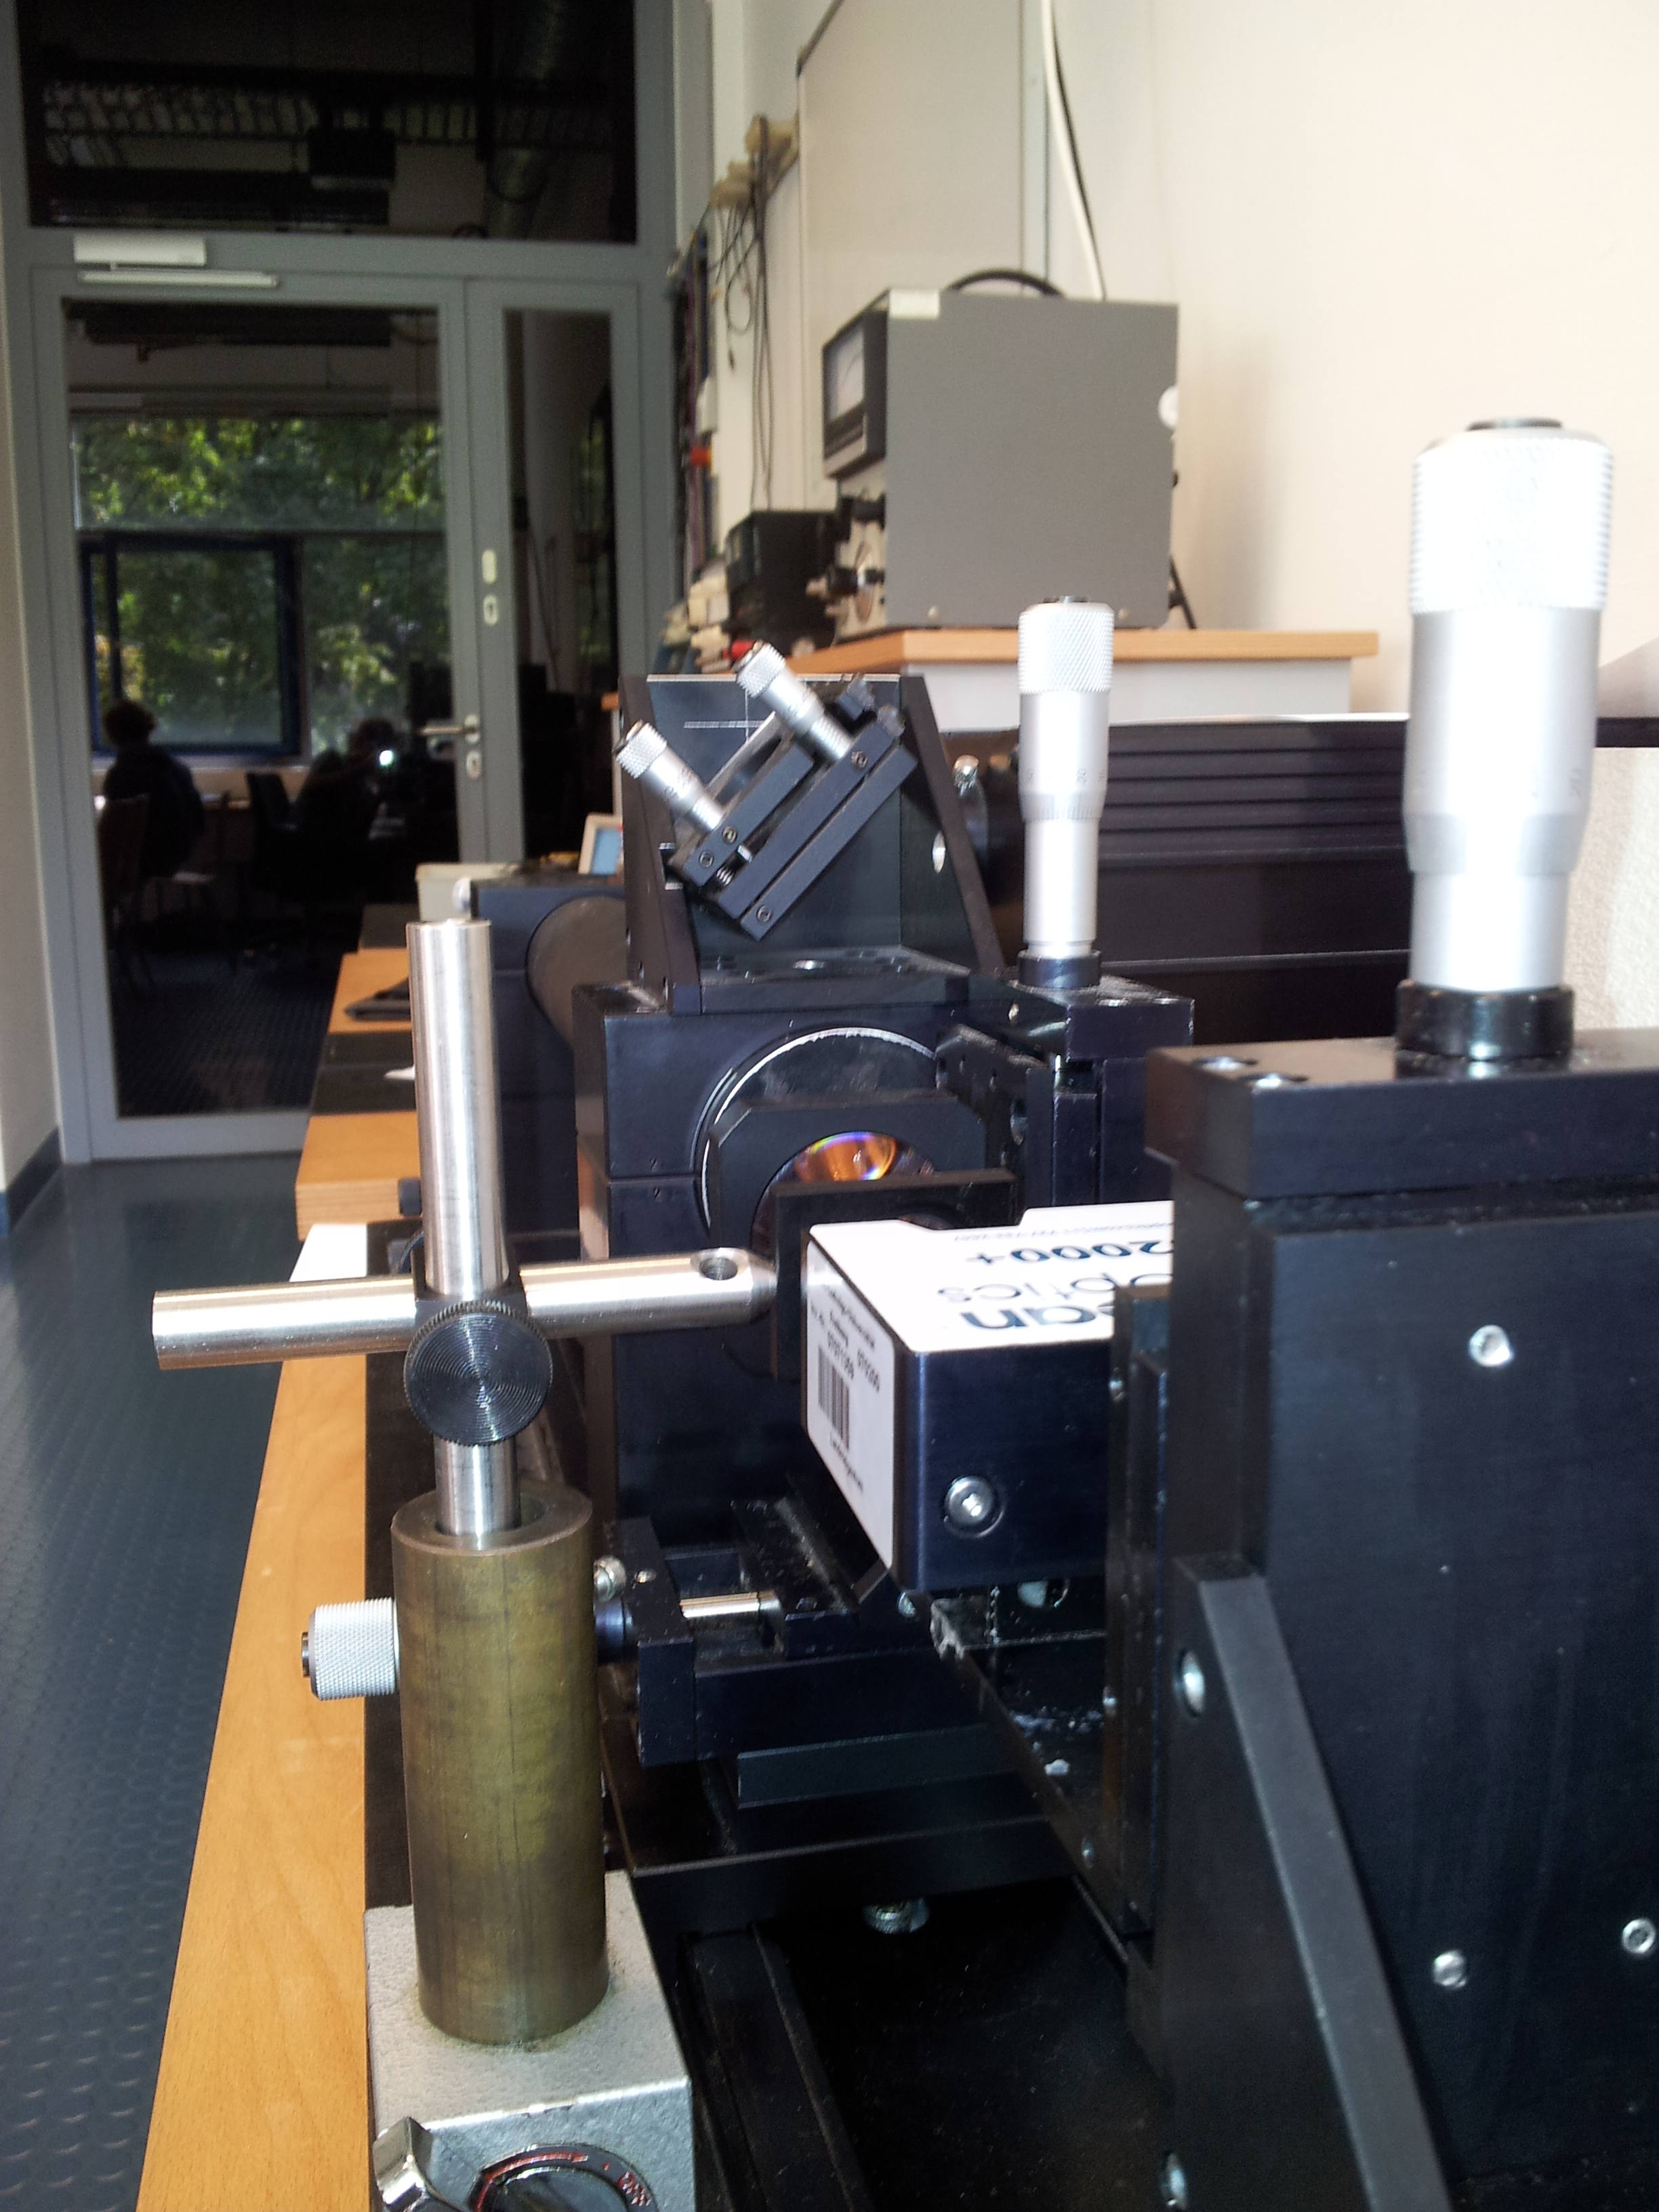
\includegraphics[width=6cm]{pics/const3}
 \label{fig:const3}
\end{SCfigure}
sample textsample textsample textsample textsample textsample text
sample textsample textsample textsample textsample textsample text
sample textsample textsample textsample textsample textsample text
sample textsample textsample textsample textsample textsample text
sample textsample textsample textsample textsample textsample text
sample textsample textsample textsample textsample textsample text
